

\documentclass[a4paper]{article}

\usepackage{amsmath}
\usepackage{hyperref}
\usepackage{biblatex}
\usepackage{enumerate}
\usepackage{graphicx}
\usepackage{stmaryrd}
\usepackage[dvipsnames]{xcolor}
\usepackage{listings}
\usepackage{caption}
\usepackage{subcaption}
\usepackage{booktabs}


\addbibresource{refs.bib}

\begin{document}

\author{Ola Bratt \\
  \href{mailto:ola.bratt@gmail.com}{ola.bratt@gmail.com}
  \and
  Patrick Attimont \\
  \href{patrickattimont@gmail.com}{patrickattimont@gmail.com}
}

\title{DAT565/DIT407 Assignment 3}
\date{2024-02-xx}

\maketitle

This paper is addressing the assignment 3 study queries within the \emph{Introduction to Data Science \& AI} course, DIT407 at 
the University of Gothenburg and DAT565 at Chalmers. The main source of information for this project
is derived from the lectures and Skiena~\cite{Skiena:2024}. Assignment 3 is about text classification and the 
use of correct data splitting and encoding handling.

\section*{Problem 1: Spam and Ham}

\subsection*{A. Data exploration}

\subsection*{B. Data splitting}
Since we have a large dataset, we can use the \texttt{train\_test\_split} function from the \texttt{sklearn.model\_selection}. With a smaller
dataset it would be better to use cross-validation to avoid overfitting.

\begin{verbatim}
  X_train, X_test, y_train, y_test = 
  train_test_split(email_matrix, labels, test_size=0.2)
\end{verbatim}
\section*{Problem 2: Preprocessing}
The "bag of words" model is a basic and intuitive way to analyze and compare documents based on their textual content. 
However, it does not consider the context or the order of words, which can limit its effectiveness in capturing the semantics 
and meaning of the text.
\section*{Problem 3: Easy Ham}

To calculate the precision, recall, accuracy and confusion matrix, we use the following code (These functions are available in the \texttt{sklearn.metrics} package): 
\begin{verbatim}
  accuracy = accuracy_score(y_test, y_pred)
  precision = precision_score(y_test, y_pred)
  recall = recall_score(y_test, y_pred)
  conf_matrix = confusion_matrix(y_test, y_pred)
\end{verbatim}

Accuracy measure the proportion of true results among the total number of cases examined, this is calculated according to Equation~\ref{equation:accuracy}. 
Precision measures the proportion of true positive results among the total number of cases that were predicted to be positive, this is calculated according to Equation~\ref{equation:precision}. 
Recall measures the proportion of true positive results among the total number of cases that were actually positive, this is calculated according to Equation~\ref{equation:recall}.
F1 score is the harmonic mean of precision and recall, this is calculated according to Equation~\ref{equation:f1}.
These metrics are used to evaluate the performance of the models. Higher values are better.

The accuracy, precision, recall, and F1 score for the easy ham and spam dataset are shown in Table~\ref{tabular:easy_summary}. 
The confusion matrixes for the easy ham and spam dataset are shown in Figure~\ref{fig:easy_ham_and_spam_confusion_matrix}.
\begin{equation}
  \label{equation:accuracy}
  Accuracy =  \cfrac{ TP + TN}{TP + TN + FP + FN}  
\end{equation}
\begin{equation}
  \label{equation:precision}
  Precision = \cfrac{ TP}{TP + FP}  \\
\end{equation}
\begin{equation}
  \label{equation:recall}
  Recall = \cfrac{ TP}{TP + FN}  \\
\end{equation}
\begin{equation}
  \label{equation:f1}
  F1 = 2 * \cfrac{ Precision * Recall}{Precision + Recall}
\end{equation}

\begin{table}
  \begin{center}
  \begin{tabular}{ l|l|l|l|l }
    \hline
    \text{Model} & \text{accuracy} & \text{precision} & \text{recall} & \text{F1 score}\\
    \hline
    \text{Multinomial Naive Bayes} & 0.985 & 0.984 & 0.998 & 0.991 \\
    \text{Bernoulli Naive Bayes} & 0.923 & 0.918 & 0.996 & 0.956 \\
  \end{tabular}
\end{center}
\caption{Metrics for Easy Ham and Spam}
  \label{tabular:easy_summary}
\end{table}


\begin{figure}
  \centering
  \begin{subfigure}[a]{\textwidth}
      \centering
      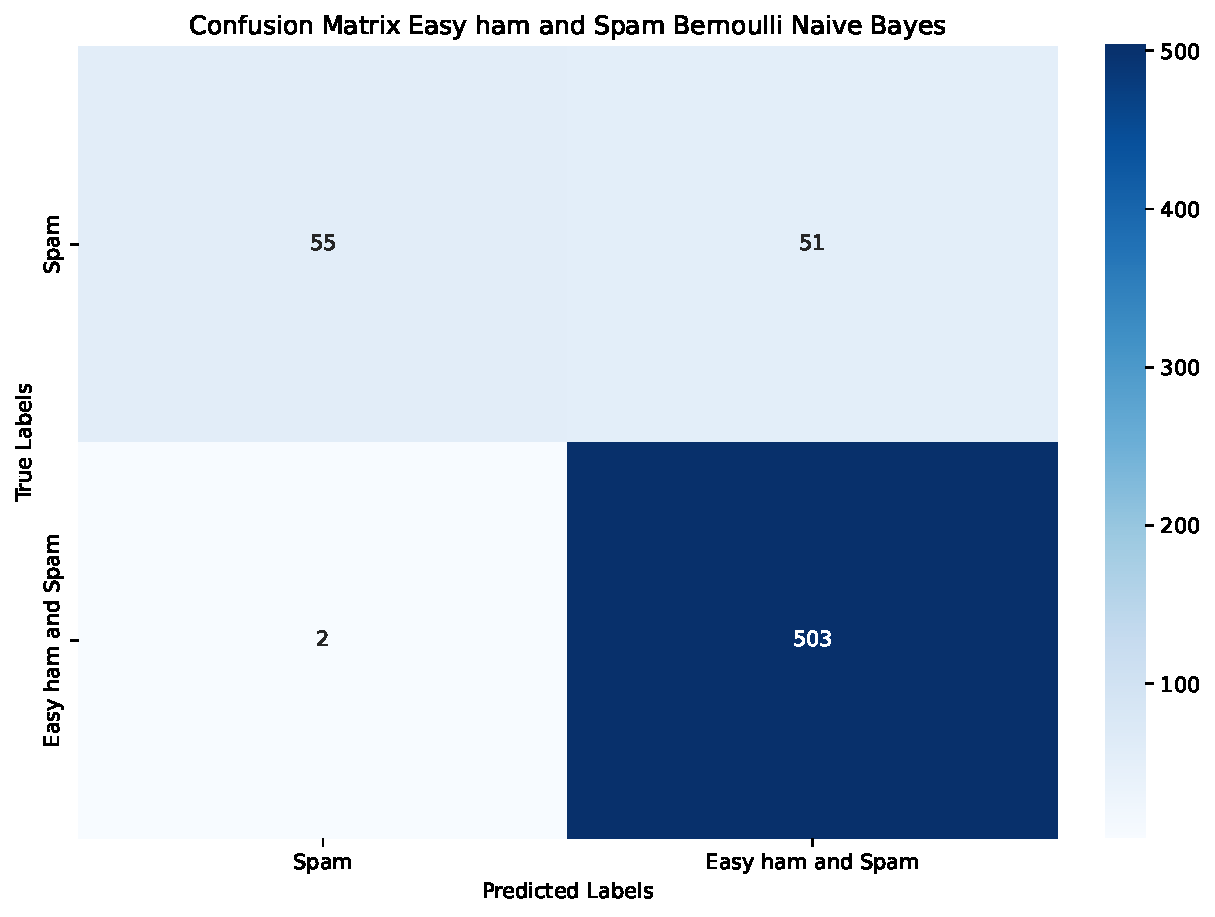
\includegraphics[width=\textwidth]{easy_ham_and_spam_bernoulli_naive_bayes_confusion_matrix.pdf}
      \caption{Easy ham vs spam, Bernoulli Naive Bayes}
      \label{fig:easy_ham_and_spam_bernoulli_naive_bayes_confusion_matrix}
  \end{subfigure}
  \vfill
  \begin{subfigure}[b]{\textwidth}
      \centering
      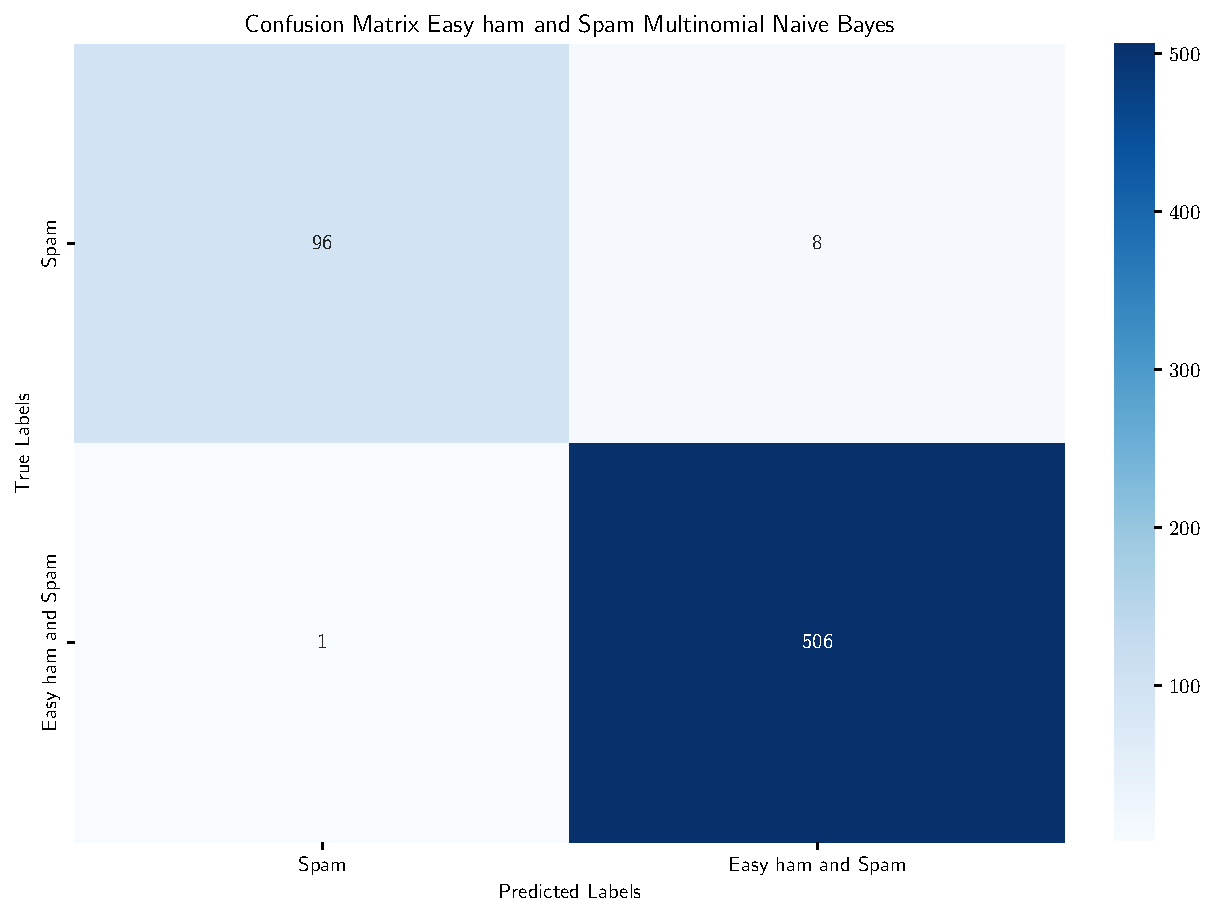
\includegraphics[width=\textwidth]{easy_ham_and_spam_multinomial_naive_bayes_confusion_matrix.pdf}
      \caption{Easy ham vs spam, Multinomial Naive Bayes}
      \label{fig:easy_ham_and_spam_multinomial_naive_bayes_confusion_matrix}
  \end{subfigure}
  \caption{Confusion matrixes of easy ham and spam}
  \label{fig:easy_ham_and_spam_confusion_matrix}
\end{figure}

\newpage
\section*{Problem 3: Hard Ham}
The accuracy, precision, recall, and F1 score for the hard ham and spam dataset are shown in Table~\ref{tabular:hard_summary}.
The confusion matrixes for the hard ham and spam dataset are shown in Figure~\ref{fig:hard_ham_and_spam_confusion_matrix}.


\begin{table}
  \begin{center}
  \begin{tabular}{l|l|l|l|l}
    \hline
    \text{Model} & \text{accuracy} & \text{precision} & \text{recall} & \text{F1 score}\\
    \hline
    \text{Multinomial Naive Bayes} & 0.947 & 0.956 & 0.878 & 0.915 \\
    \text{Bernoulli Naive Bayes} & 0.934 & 0.976 & 0.816 & 0.889 \\
  \end{tabular}
\end{center}
\caption{Metrics for Hard Ham and Spam}
  \label{tabular:hard_summary}
\end{table}

\begin{figure}
  \centering
  \begin{subfigure}[a]{\textwidth}
      \centering
      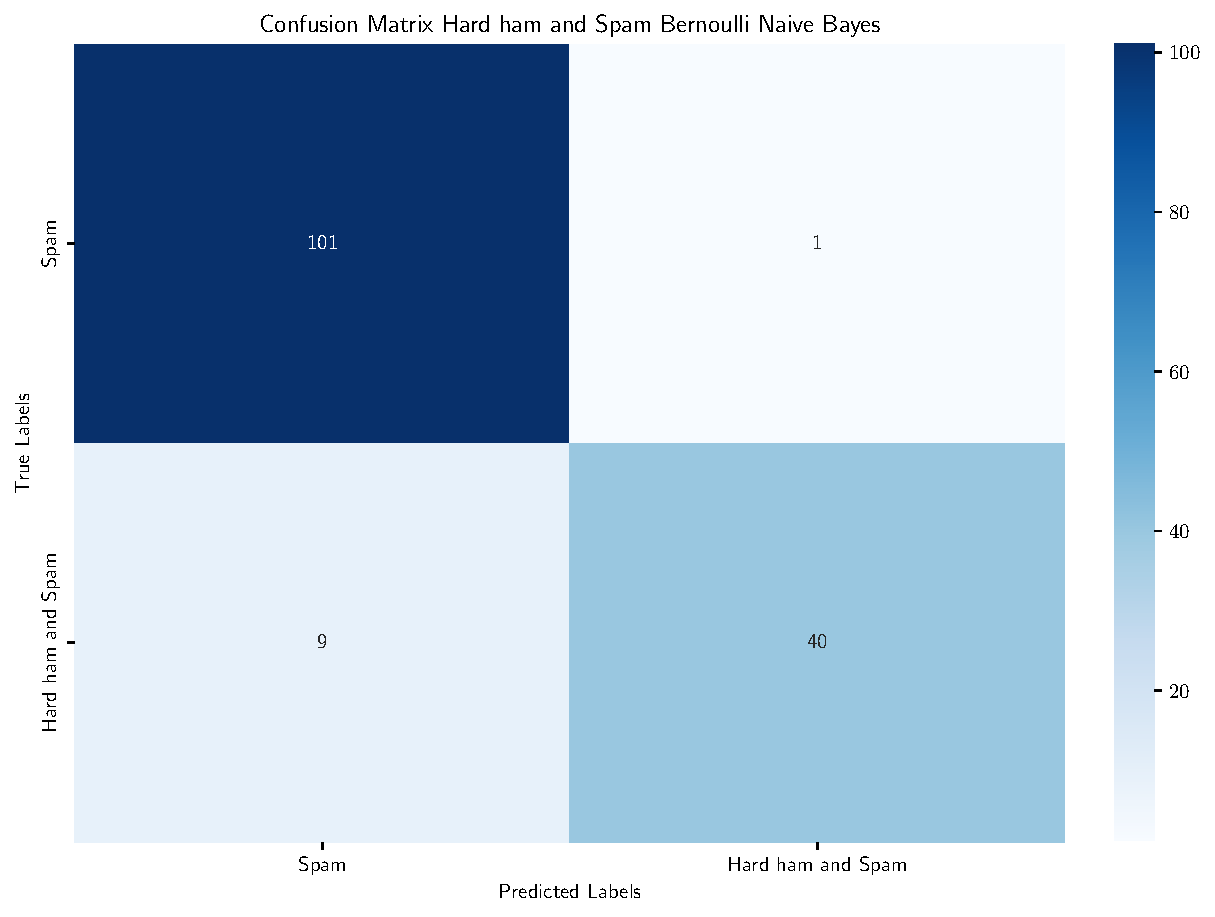
\includegraphics[width=\textwidth]{hard_ham_and_spam_bernoulli_naive_bayes_confusion_matrix.pdf}
      \caption{Hard ham vs spam, Bernoulli Naive Bayes}
      \label{fig:hard_ham_and_spam_bernoulli_naive_bayes_confusion_matrix}
  \end{subfigure}
  \vfill
  \begin{subfigure}[b]{\textwidth}
      \centering
      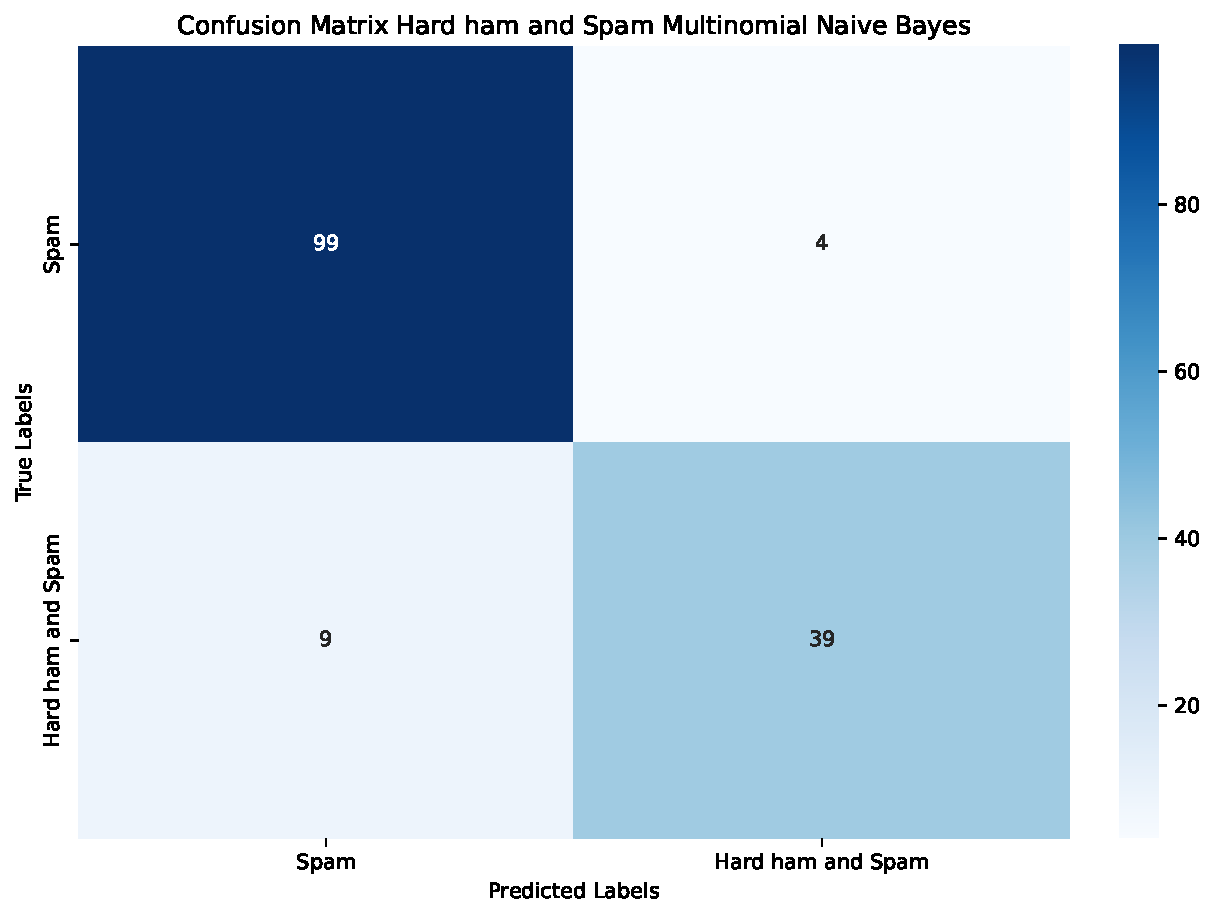
\includegraphics[width=\textwidth]{hard_ham_and_spam_multinomial_naive_bayes_confusion_matrix.pdf}
      \caption{Hard ham vs spam, Multinomial Naive Bayes}
      \label{fig:hard_ham_and_spam_multinomial_naive_bayes_confusion_matrix}
  \end{subfigure}
  \caption{Confusion matrixes of hard ham and spam}
  \label{fig:hard_ham_and_spam_confusion_matrix}
\end{figure}

\newpage





\printbibliography

\section*{Appendix: Source Code}

\lstset{
  language=Python,
  basicstyle=\ttfamily,
  commentstyle=\color{OliveGreen},
  keywordstyle=\bfseries\color{Magenta},
  stringstyle=\color{YellowOrange},
  numbers=left,
  basicstyle=\footnotesize,
  breaklines=true,
  postbreak=\mbox{\textcolor{red}{$\hookrightarrow$}\space}
}


\lstinputlisting{ola/assignment3.py}

\end{document}
